\documentclass[12pt,a4paper]{article}
\usepackage[pdftex]{graphicx}
\usepackage{url} 
\usepackage[bookmarks, colorlinks=false, pdfborder={0 0 0}, pdftitle={<pdf title here>}, pdfauthor={<author's name here>}, pdfsubject={<subject here>}, pdfkeywords={<keywords here>}]{hyperref} 
\usepackage{caption}
\usepackage{subcaption}
\usepackage{float}
\usepackage{amsmath} % for math and matrix formulations.
\usepackage[section]{placeins}

% Paper margins etc.
\usepackage{geometry}
 \geometry{
 a4paper,
 total={160mm,257mm},
 left=25mm,
 top=25mm
 }

\begin{document}

\begin{titlepage}

\begin{center}


\includegraphics[width=0.3\textwidth]{Figures/metu_logo.png}\\
\vspace{.3in}
\textup{{\bf Middle East Technical University}}\\

% Title
\Large \textbf{EE463 Static Power Conversion I}\\[0.3in]
\Large \textbf{Term Project}\\
\Large \textit{Complete Simulation Report}\\

\noindent\rule{6cm}{0.4pt}

% Authors
\normalsize \textit{Submitted by:} \\

\textbf{Işık Emir Altunkol}\\
\textbf{ID:2442408}\\
emir.altunkol@metu.edu.tr\\
\textbf{tel:531 320 04 43} \\

\vspace{.3in}

\textbf{İsmail Macit}\\
\textbf{ID:2305084}\\
ismail.macit@metu.edu.tr\\
\textbf{tel:539 678 03 96} \\

\vspace{.3in}

\textbf{Fatih Erden}\\
\textbf{ID:}2304566\\
fatih.erden@metu.edu.tr\\
\textbf{tel:} 533 895 38 07\\

\noindent\rule{6cm}{0.4pt}

\vspace{.3in}

\textbf{Submission Date:} 10.12.2022

\end{center}

\end{titlepage}

\pagenumbering{arabic}

\tableofcontents

\newpage
\listoffigures
\listoftables

\newpage
\section{Introduction} \label{intro}

Starting of DC motors can be tricky in many applications. Basic modelling of DC motors can be given in following figure and equations:

\begin{figure}[ht!]
    \centering
    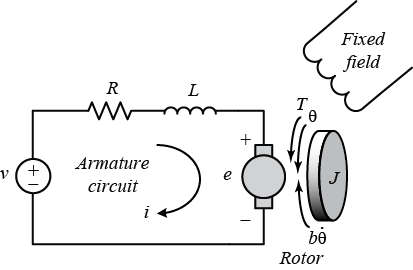
\includegraphics{Figures/DC_motor_model.png}
    \caption{Simplified DC-machine model.}
    \label{fig:DC-mmotor}
\end{figure}

\begin{equation}
    E_{emf} = K_e\times\omega
\end{equation}

\begin{equation}
    T_e = K_t\times I
\end{equation}

where $K_e$ and $K_t$ are machine constants. $\omega$ being the machine rotational speed, at the starting operation, it is obviously zero. Therefore if we apply a high DC voltage at the starting instant, the DC machine will draw high amounts of currents which can damage the device, permanently. To prevent this possibility, one can start the DC motor in a proper way, not applying a step voltage (rated) to the motor terminals, but rather applying a voltage that increases properly up to the rated value. This kind of operation is called \textit{soft start} and it is helpful  in prolonging the lifetime of the DC motor. In this project, our aim is to make a rectifier controller that is capable of soft-starting the DC motor. Requirements of the controllers and details of the motor of interest are given on course Github web page.\cite{course_git} These will also be used in the following sections of the report.

There are different types of topologies for this purpose of soft start. Some of the common topologies are discussed and evaluated on the issues of efficiency, operation regions and ratings, component availability, thermal and mechanical considerations, etc. on the design decision in \ref{design}. Also, the reasons behind the  design selection of Hard-time Regulators are given in the same section. Selected topology is simulated on computer software programs and the performance of the topology is investigated in the related section \ref{simulations}. Also, possible components that are commercially available and appropriate for the design, are issued on the component selection (see \ref{component}). Summary and future considerations on the design are given in the conclusion.(see \ref{conclude})

\newpage
\section{Design Decisions} \label{design}
In this section, comparison of different topologies and the decision process of our team are given. The advantages of the selected topology, reasons behind it, possible difficulties that can occur during the process are discussed. Controlling of the selected topology and signal and interactions between the modules of the design are explained in the following subsection. Then mechanical and thermal issues of the design are discussed. Possible solutions to the stability and heating problems of the design are proposed. Finally connection and measurement ports of the device for application and testing are discussed. 

\subsection{Topology Selection}

There are common topologies like thyristor rectifiers (three-phase or single-phase) for rectifying AC input and controlling the DC-output at the same time. By controlling the firing angles ($\alpha$) of the thyristors, one can adjust the voltage levels of the output voltage. A topology given in Figure \ref{fig:single_phase_thyristor_fb} is an example to this topology. As it can be seen in the figure, 4 thyristors are to be controlled with their $\alpha$ firing angles. In three-phase case of the same topology, this 6 thyristors are to be controlled. However, this configuration does not support 4 quadrant operation of the DC motor since the thyristors allow only way for the current to flow. To achieve the 4 quadrant operation, one can replace each thyristor with back-to-back two thyristors, which can be seen in Figure \ref{fig:triac}. Control of this configuration is again more complex. \\

\begin{figure}[H]
    \centering
    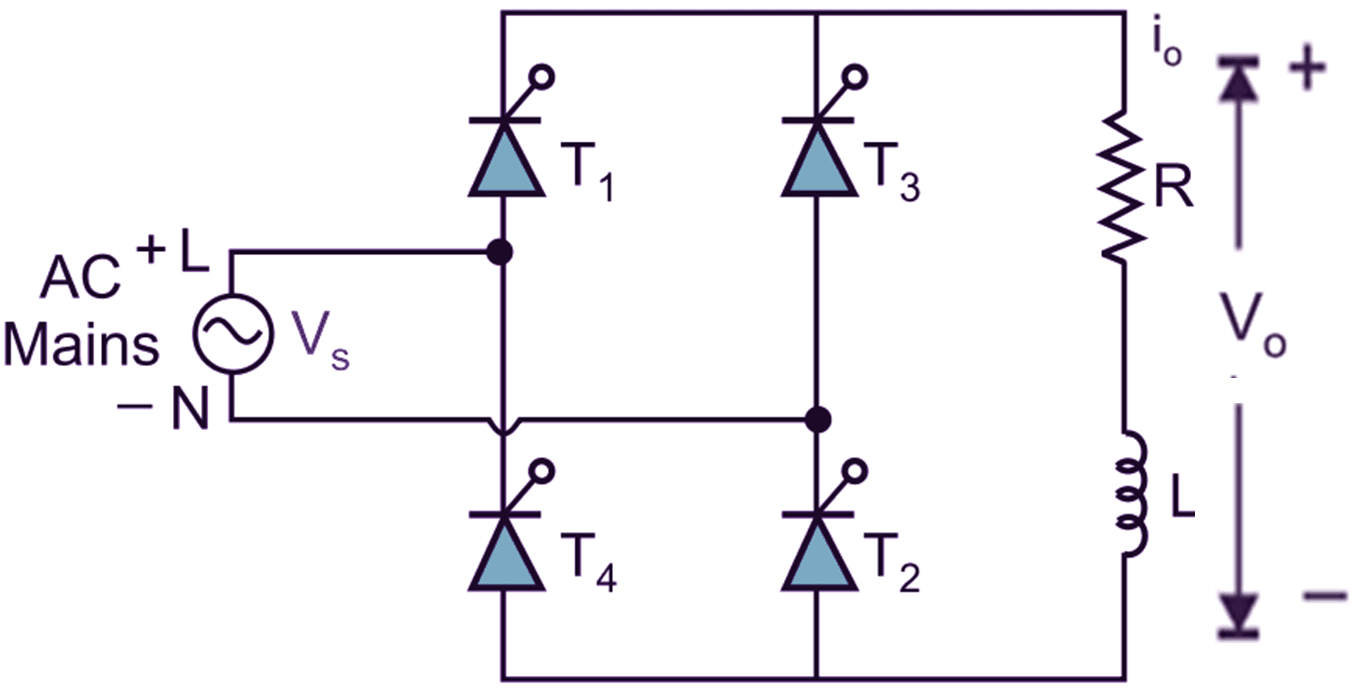
\includegraphics[width=0.7\textwidth]{Figures/single_phase_full_bridge_thyristor.png}
    \caption{Single-phase full bridge thyristor rectifier.}
    \label{fig:single_phase_thyristor_fb}
\end{figure}

\begin{figure}[H]
    \centering
    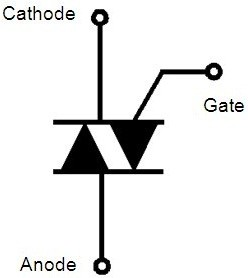
\includegraphics[width=0.2\textwidth]{Figures/triac_symbol.png}
    \caption{Back-to-back thyristors (triac).}
    \label{fig:triac}
\end{figure}

One can also use a diode rectifier (3-phase or single phase) before the DC-DC converter. In second case, only the DC-DC converter is controlled for the output voltage level. Since the maximum value of the desired output DC voltage is 180 V, a buck converter will be suitable for this case. However this topology works only in one quadrant due to the unavailability of negative duty cycles and one way allowance of the diode. To achieve the 4-quadrant operation, one alternative is the H-bridge coming after the diode rectifier. By adjusting the duty cycles of appropriate switches for desired quadrant of operation, one can drive the DC motor in all regions. Our motor drive will be designed to support 4-quadrant operation. Therefore, the topology which includes full-bridge diode rectifiers and H-bridge controller is selected to be implemented. Overall configuration of the design that will drive the DC motor is given in the Figure \ref{fig:overall_diagram}. In generation modes, armature current flowing to the driver will be dissapated through a chopper resistance which is also controlled by a switch to utilize its operation. \\


\subsection{Control Methodology}
We will use PWM (Pulse Width Modulation) signals to control the MOSFETs, which will control the average voltage seen in the output terminals. We will use a micro-controller to generate and regulate the PWM signals according to the user input and system state. To drive the MOSFETs with the micro-controller signals, we need to use gate driver circuits. We will use an Arduino controller (ATMegaxxx) as microcontroller, and commercial half-bridge gate drivers will be ordered and used directly to reduce the circuit design workload and have better performance. \\

To be able to soft-start the DC-motor, avoid the armature current ripple, and avoid high transient currents during reference input changes, we will need a closed loop control methodology between DC-motor terminal voltage and the duty cycles of the switches (MOSFETs). If we do not control the terminal voltage and apply PWMs with constant duty cycles, motor will experience huge amount of torques (inducing high currents on the armature) that will damage the DC-motor and decrease its lifetime. Figure \ref{fig:overall_diagram} shows the overall control topology of the DC-motor driver design. Overall, the design does not control the rectifier side of the motor drive, full-bridge diode rectifiers are used to rectify the AC input. Then the ripple at the DC-output will be suppressed by an appropriate shunt capacitor. To be able drive the DC-motor on the generating modes, team decided not to supply the energy to the grid side, since the design does not have an inverter that will generate AC to be supplied to the grid. Instead, there will be open terminals for chopper resistance that will dissipate the supplied power when the DC-machine operates in generating modes. And then, depending on the operation mode, the controller will send the required PWM duty cycles to the gate drivers of the switches. Detailed information about the closed loop controls of switches are given below.

\begin{figure}[H]
    \centering
    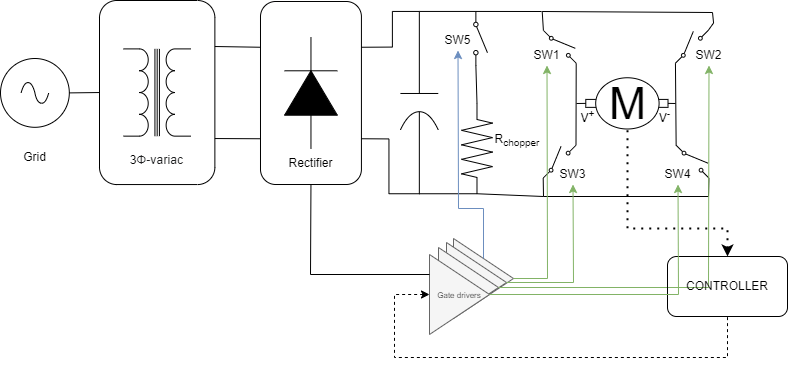
\includegraphics[width=0.8\textwidth]{Figures/topology_deneme.png}
    \caption{DC-motor drive system diagram.}
    \label{fig:overall_diagram}
\end{figure}

In our design, we plan to use closed-loop current control to control our driver by implementing a PID (Proportional Integral Derivative) controller. Since the armature current increases with increasing duty, it can be controlled by changing the duty cycles of the switches. The duty cycles will be adjusted using an error signal. By taking the discrete time derivative and integral of this error signal, we may obtain a discrete time PID controller. The equation for controlling the current by adjusting the duty cycle is given in Equation \ref{eqn:PID}.

\begin{equation}
    \begin{split}
        \Delta D = K_pE_{I_a} + K_i\sum_{n=1}^{t} E_{I_a}\Delta t + K_d\frac{\Delta E_{I_a}}{\Delta t}
    \end{split}
    \label{eqn:PID}
\end{equation}
\\
\subsection{Mechanical, Thermal, and Isolation Considerations}

In order to protect the DC-motor driver design from external incidents and achieve safer operation for users, the design will be enclosed in a 3D printed box. The size and shape of the box will be appropriate for industrial design applications. According the component sizes and PCB dimensions, smallest box volume will be selected and the DC-motor drive will be fixed in the volume. \\

Placement and connections of the components of the DC-motor drive will be solved on the PCB. This will prevent possible human-made errors and resulting parasitic effects on the circuit. It will also ease the industrial production of the design. \\

After the component selection and their trials during the implementation process, the conduction and switching losses will be calculated, compared with their simulation counterparts, then a proper-sized heatsink will be placed where the most of the heat losses occur on the circuit. \\

To prevent the motor driver circuit from possible loops that will endanger the operation of components, some isolation is required between the power flow lines and signal lines of the circuit and gate drivers. Therefore, the use of optocouplers are to be implemented on the design.

\subsection{Other Considerations}

To make the design available for easy use and proper testing, connection and measurement ports will be added to the design. According to the rated values (current and voltage) of the power lines, required isolation and line thicknesses will be implemented on both the connection ports and the PCB. For input power connection, proper sized banana plugs as seen in Figure \ref{fig:banana} can be selected. According to the connection style of DC-motor to be driven, again proper style of power cables for the output ports, will be selected.

\begin{figure}
    \centering
    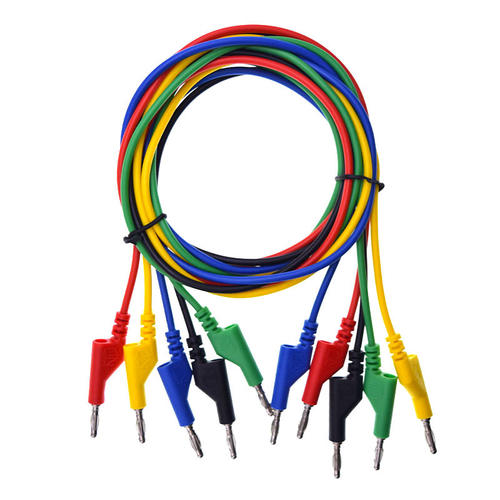
\includegraphics[width=0.4\textwidth]{Figures/banana plugs.jpg}
    \caption{Banana plug power cables for input side.}
    \label{fig:banana}
\end{figure}

For the measurement ports, the information on test procedures will be requested. Already selected ports for measurements are input and output voltages, ground connection of the motor drive. Since a series connection is requested for the electrical power calculations, it is assumed that power measurements will be taken before the input and output connections. If it is requested, the measurement ports for PWM signals of the gate drivers can be brought into the open. \\

To protect the components from over-voltages and over-currents during the operation, below measures can be applied to the design:

\begin{itemize}
    \item Fuses or current sensors at both the input and output sides of the driver circuit is thought to be implemented for over-current protection. If current sensors are to be implemented on the design, some alarm signal is to be presented to the user through some led or control method can be implemented to cut the power of the circuit.
    \item Since we are asked to supply around 2 kW power through the motor driver (excluding losses), we are dealing with high levels of current and power that can be harmful to a human body. Therefore, proper insulation will be placed on the power lines, ports, and around the equipment.
    \item To cancel the parasitic effects of the non-idealities of the components, proper countermeasures will be considered.
\end{itemize}

\newpage
\section{Computer Simulations} \label{simulations}

\subsection{LTspice Simulations}
Since the 4-quadrant operation and control of the H-Bridge topology is not simple, we made comprehensive simulations using LTspice.A brief description of those and their results will be explained in this subsection. First, the simulation model will be described. \\

The model for the topology we are using is given in Figure \ref{fig:LTspice_topology_sch}. MOSFET models are chosen from the libraries of LTspice, whose ratings are compatible with our operation ranges. To simulate the rectified DC voltage on the input side, we occasionally used an ideal DC source to simplify the results by avoiding the input voltage ripple. We used a diode to model the one-directional current flow of the rectifier, and a capacitor to model the output filtering capacitor of the rectifier. The chopper and the H-Bridge is model is rather straightforward.

\begin{figure}[H]
    \centering
    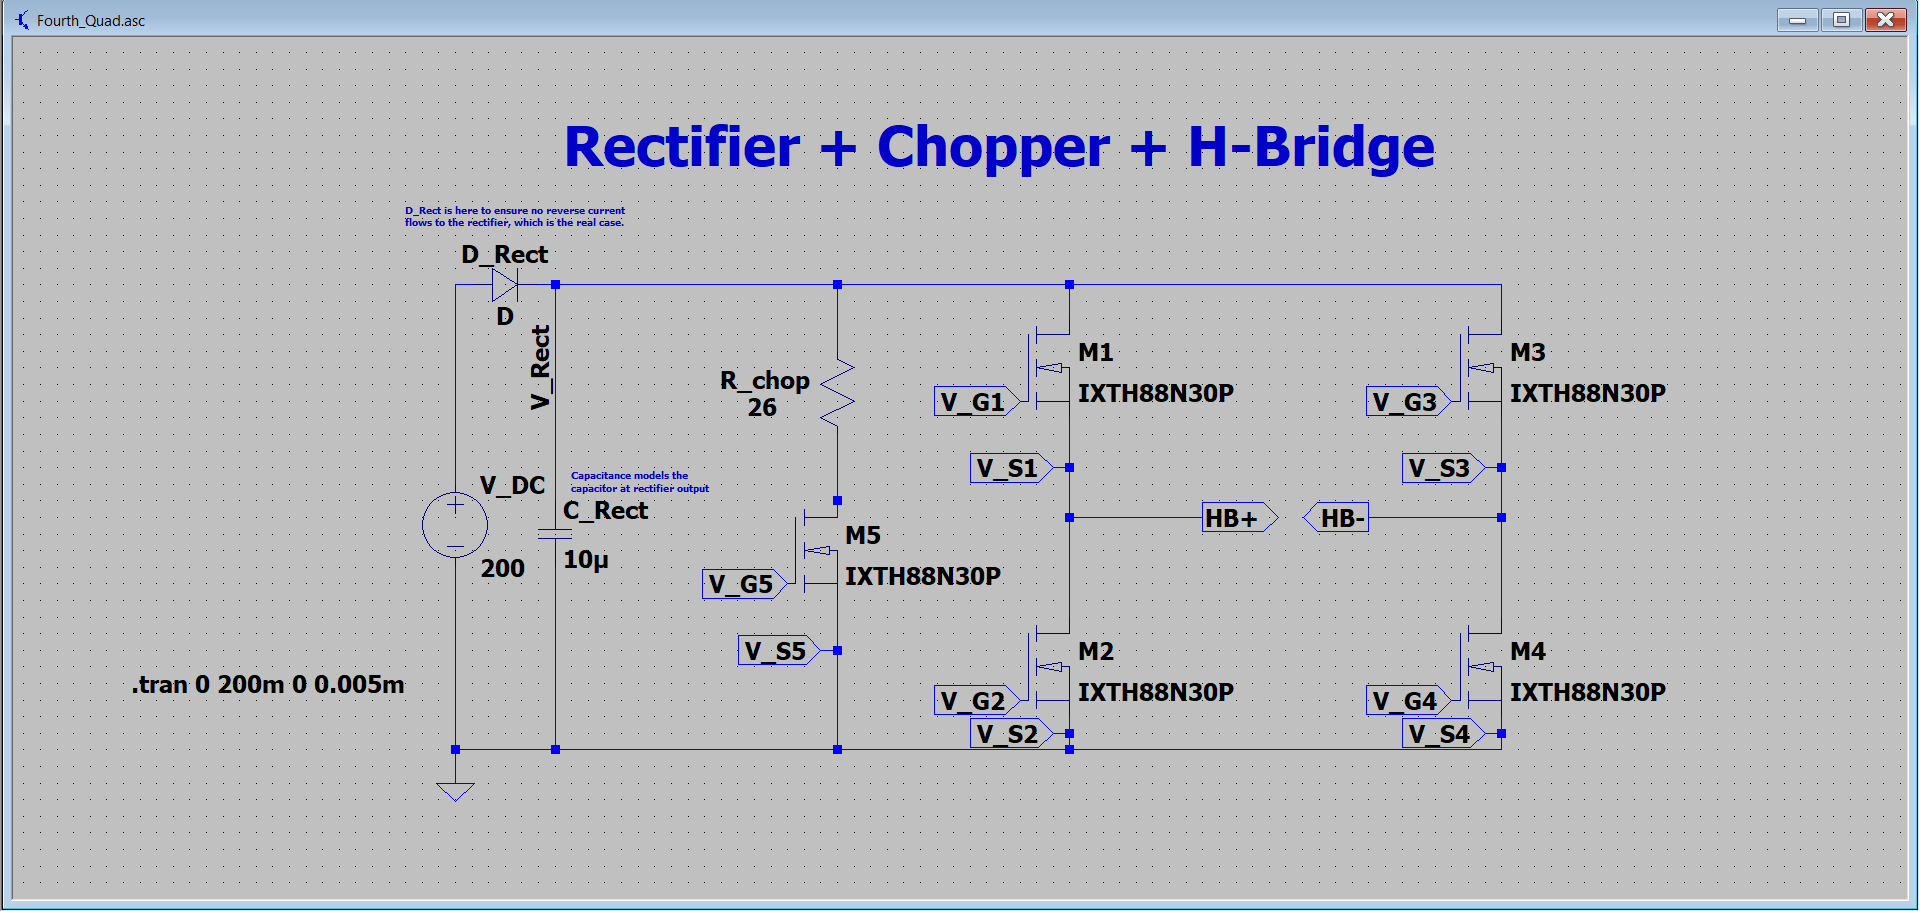
\includegraphics[width=0.8\textwidth]{Figures/Spice_Figures/Schematics/Rectifier_Chopper_H-Bridge_Schematic.PNG}
    \caption{Simulation model for the 4-quadrant motor driver topology we choose}
    \label{fig:LTspice_topology_sch}
\end{figure}

The controller and gate driver sections in Figure \ref{fig:LTspice_driver_controller_sch} are modeled using behavioral and usual voltage sources to create the necessary gate to source voltages.

\begin{figure}[H]
    \centering
    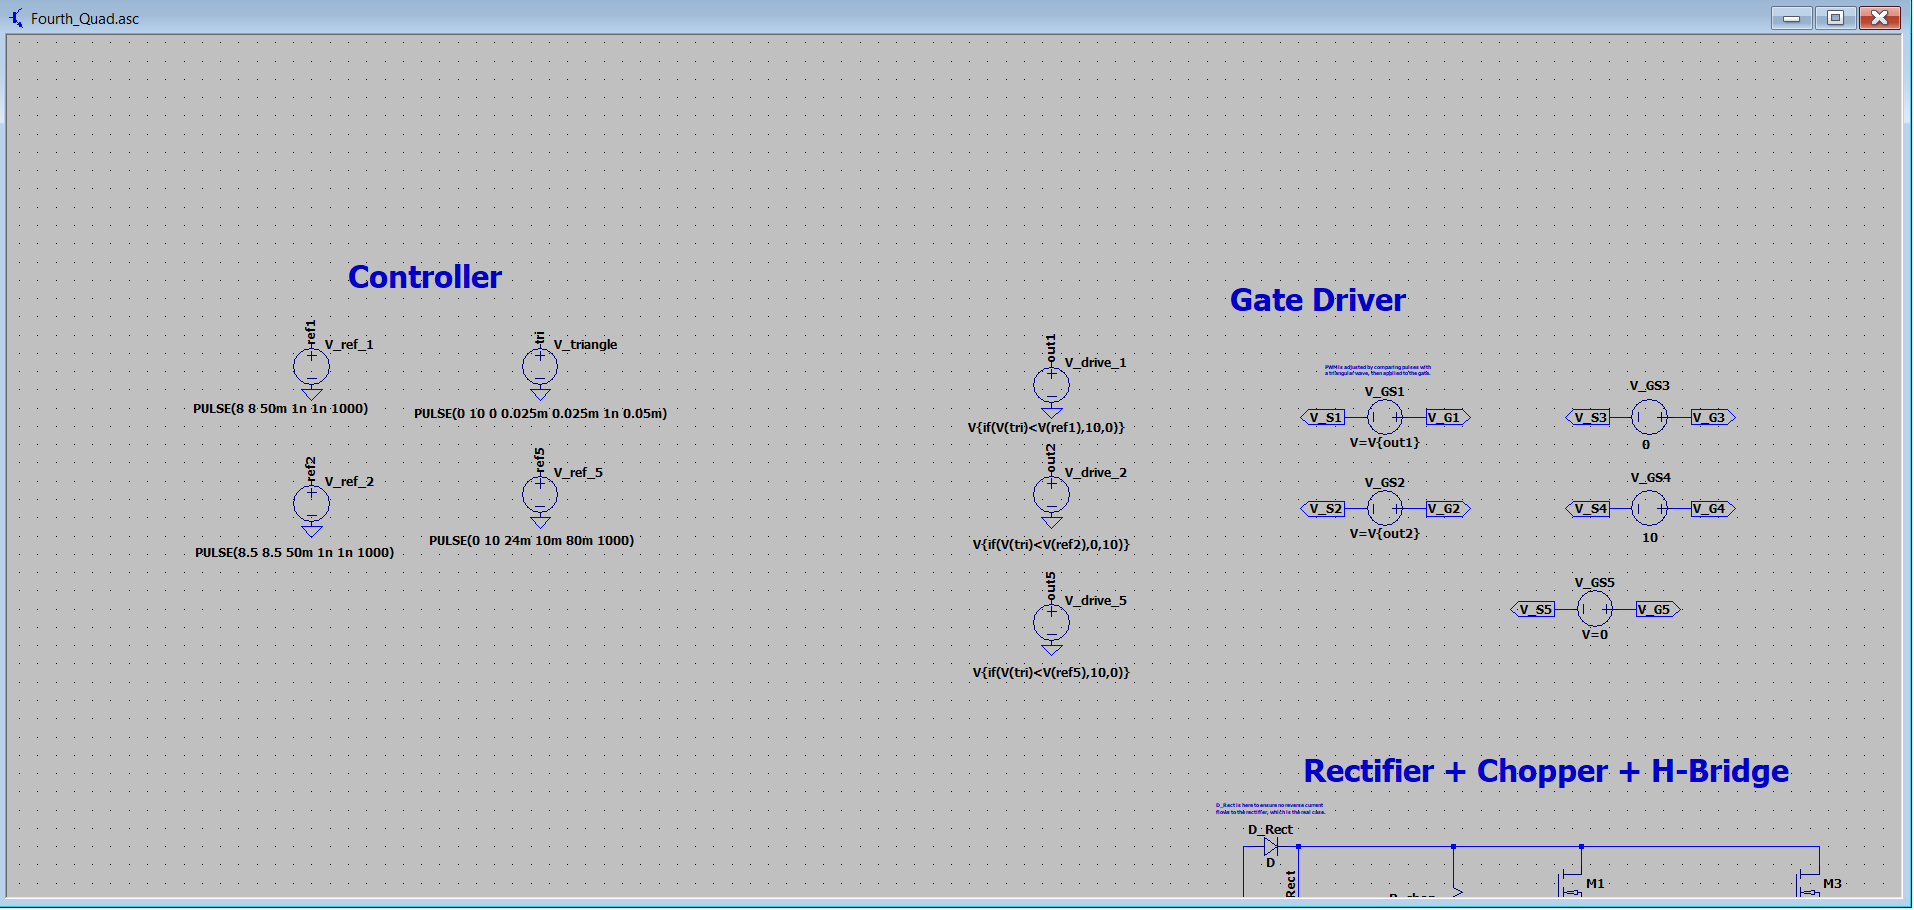
\includegraphics[width=0.8\textwidth]{Figures/Spice_Figures/Schematics/Gate_Driver_Controller_Schematic.PNG}
    \caption{A simple model to simulate the gate driver and controller operation}
    \label{fig:LTspice_driver_controller_sch}
\end{figure}

The electromechanical simulation models for DC motors are given in Figure \ref{fig:LTspice_motor_sch}. Since the simple model of the DC motor is also LTI (Linear Time Invariant), we can simulate it using the LTI circuit which is built and shown in the figure. The model can be derived using the mechanical laws for rotational systems, the torque and back emf formulas of the DC motor models, and Kirchoff's circuital laws. The motor parameters are not the final values, but found iteratively to simulate the DC motor we used as realistically as possible. Note that another DC machine is coupled to our DC machine which is going to be the The overall model for the LTspice simulations is given in Figure \ref{fig:LTspice_whole_sch}.

\begin{figure}[H]
    \centering
    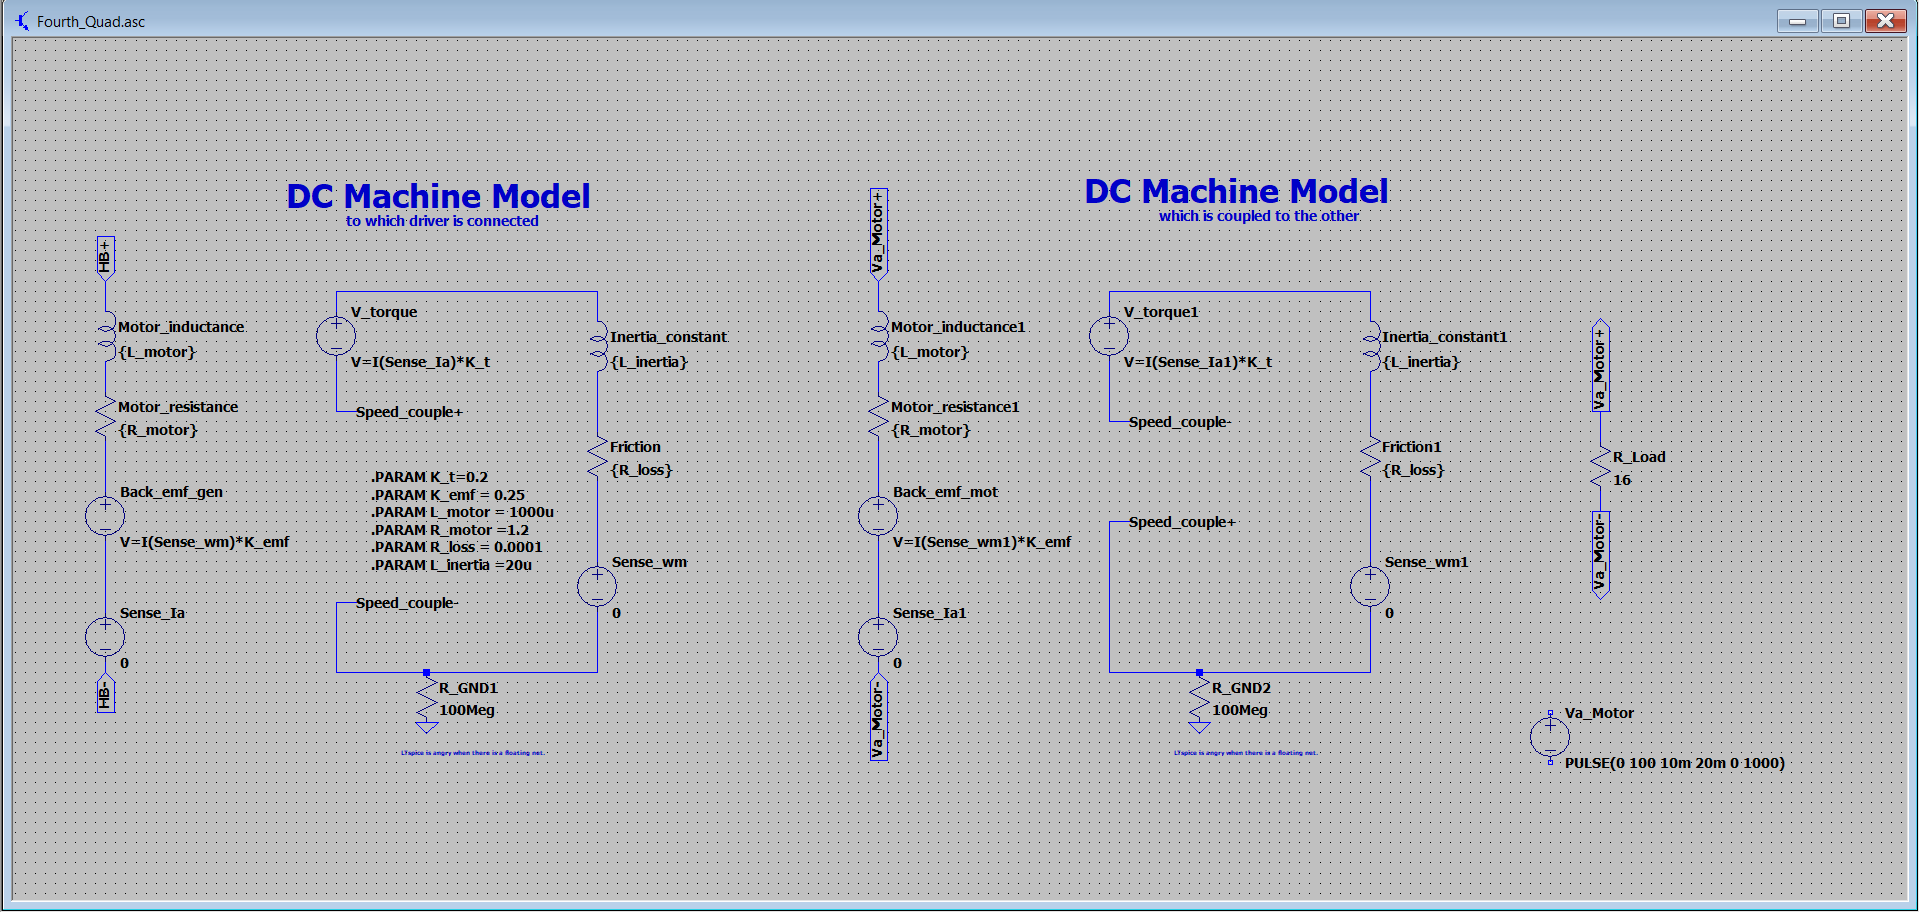
\includegraphics[width=0.8\textwidth]{Figures/Spice_Figures/Schematics/DC_Motor_Models_Schematic.PNG}
    \caption{Electromechanical simulation model for DC motors}
    \label{fig:LTspice_motor_sch}
\end{figure}

\begin{figure}[H]
    \centering
    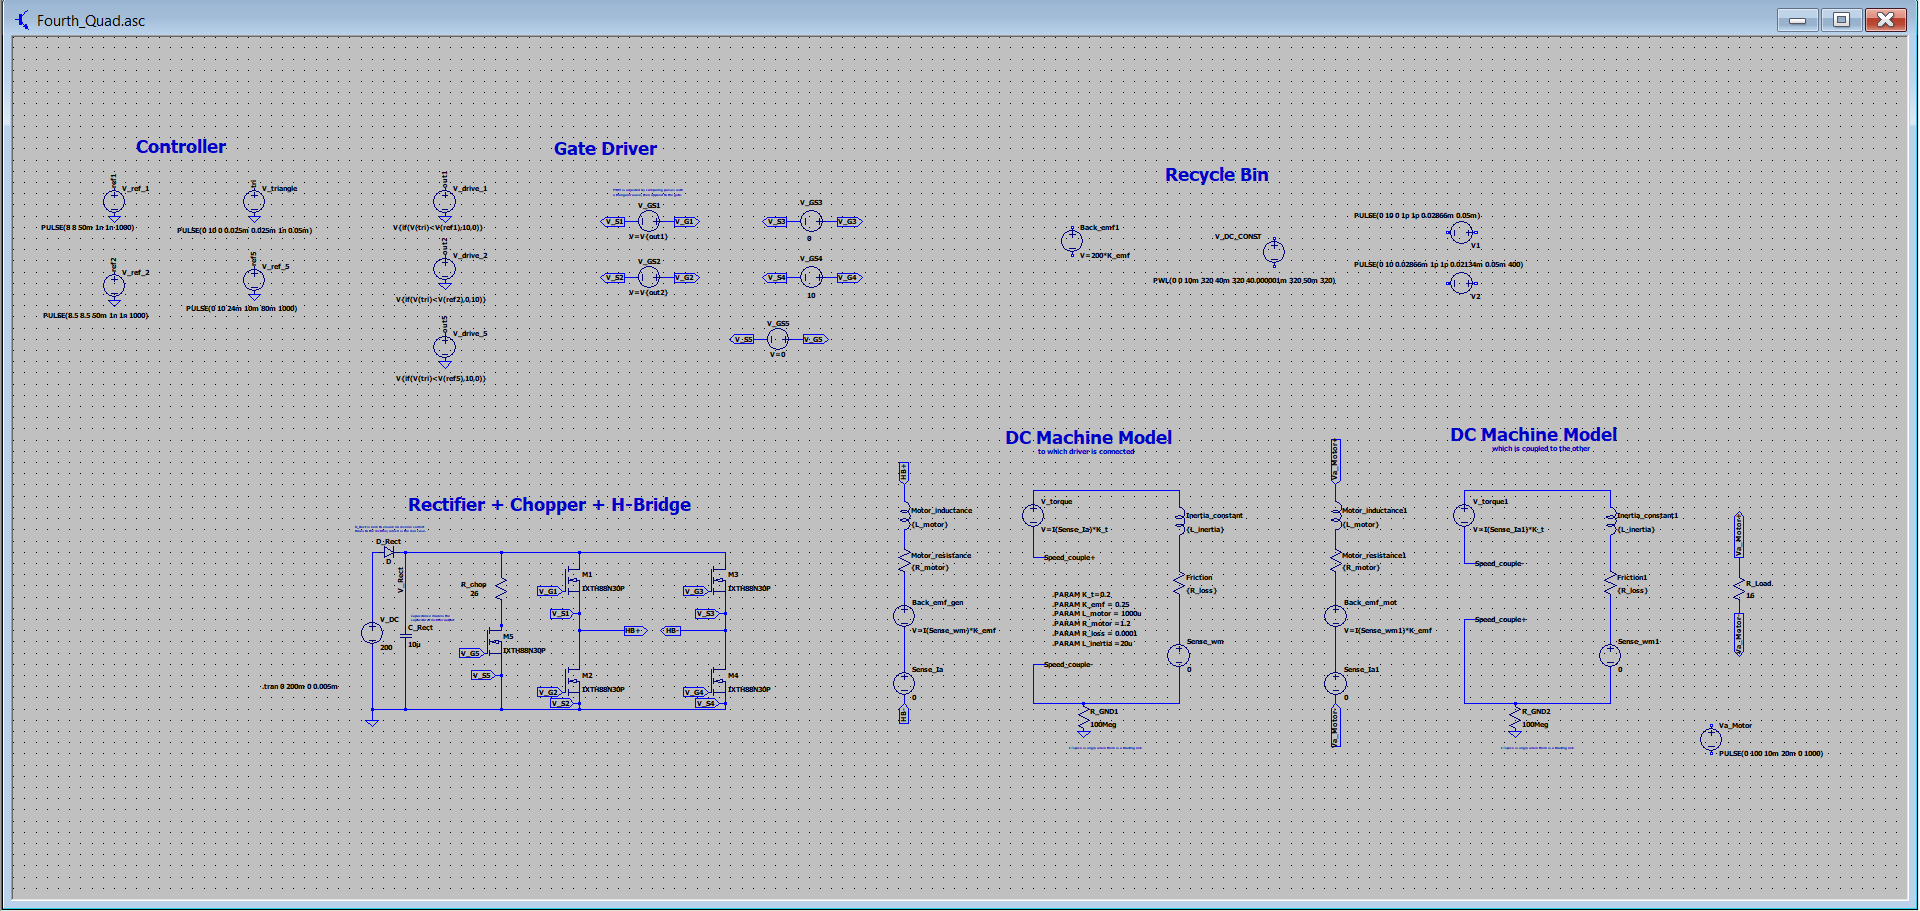
\includegraphics[width=0.8\textwidth]{Figures/Spice_Figures/Schematics/Whole_Model_Schematic.PNG}
    \caption{The complete simulation model used for the DC motor drive simulations in LTspice}
    \label{fig:LTspice_whole_sch}
\end{figure}

For the forward motoring region simulations, M1 and M2 MOSFETs are used for switching, M3 is always off, and M4 is always on for H-Bridge to operate as a synchronous buck converter. The output voltage level is directly proportional with the duty cycle of M1. For example, for 90\% duty, we obtain 180V average voltage on the motor terminals, and we obtain 100V for 50\% duty. These cases are simulated and shown in Figures \ref{fig:LTspice_forward_90_duty} and \ref{fig:LTspice_forward_50_duty}. The current on the 16 $\Omega$ load, the armature current, and the voltage on the H-Bridge terminals are given in the figures. Note that for these values, one can supply more than 2kW power with the motor driver. Hence, current and voltage ratings of the MOSFETs can be determined using such a simulation (keeping the other practical effects in mind).

\begin{figure}[H]
    \centering
    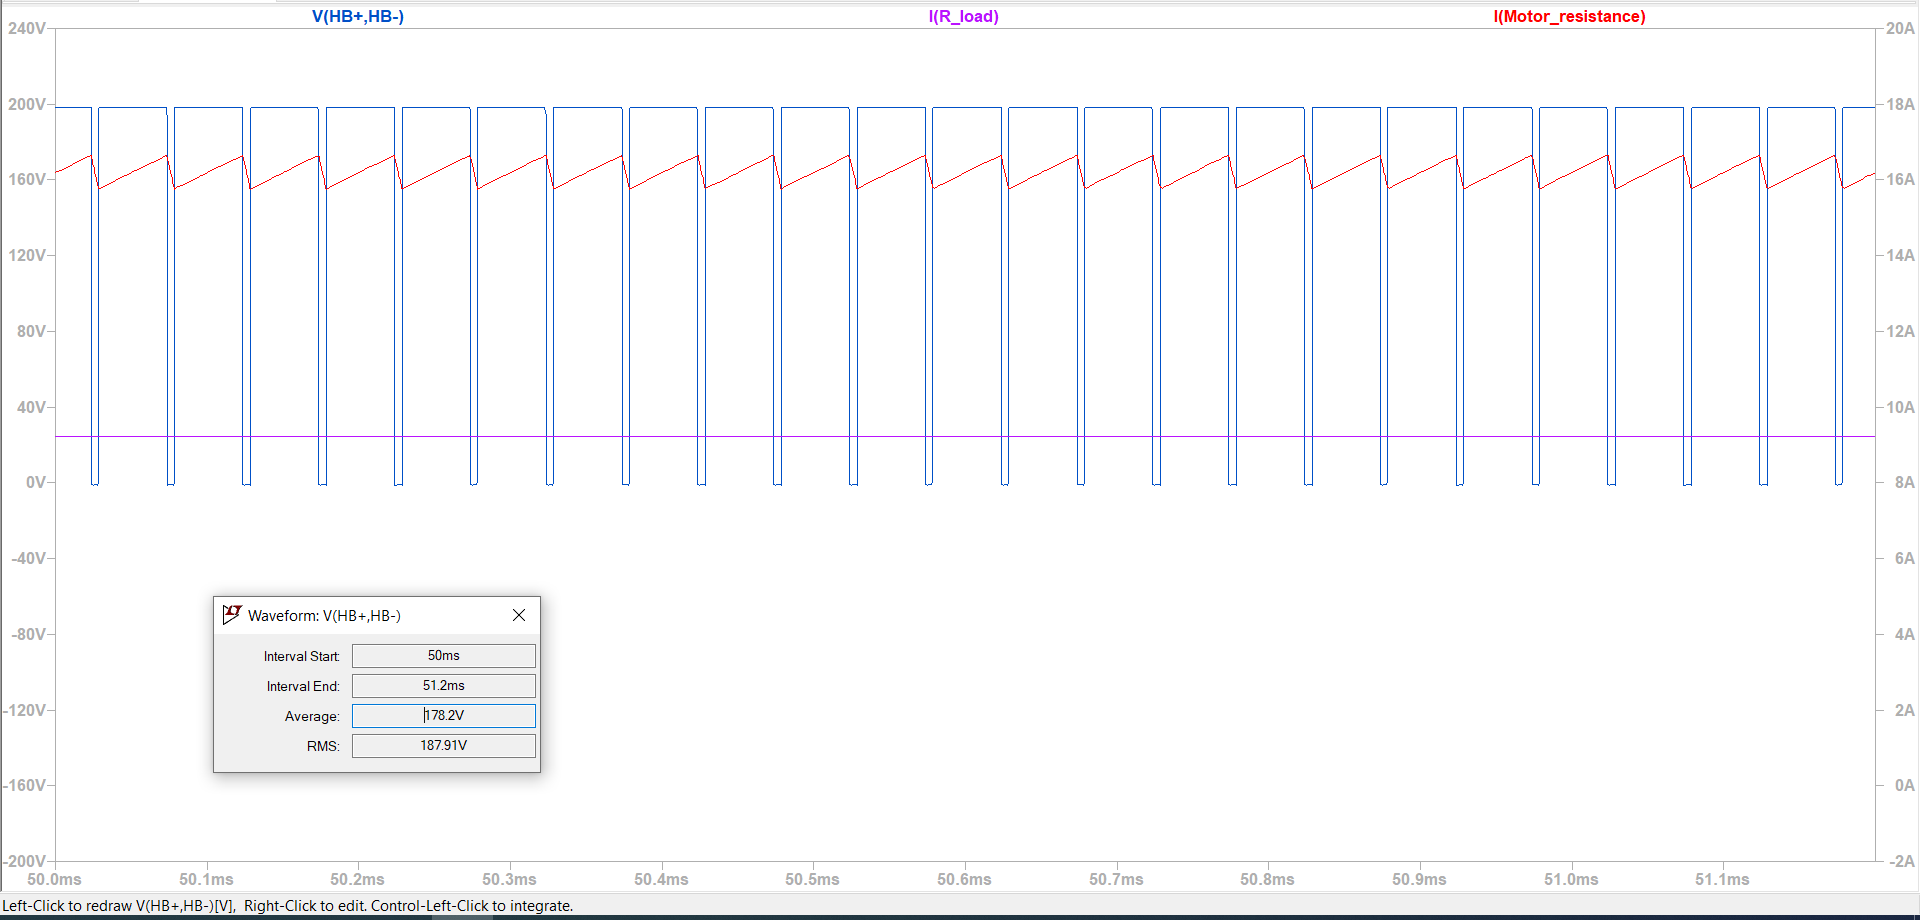
\includegraphics[width=0.8\textwidth]{Figures/Spice_Figures/Motoring_Full_Duty_Sim_1.PNG}
    \caption{Forward motoring simulation for 90\% duty}
    \label{fig:LTspice_forward_90_duty}
\end{figure}

\begin{figure}[H]
    \centering
    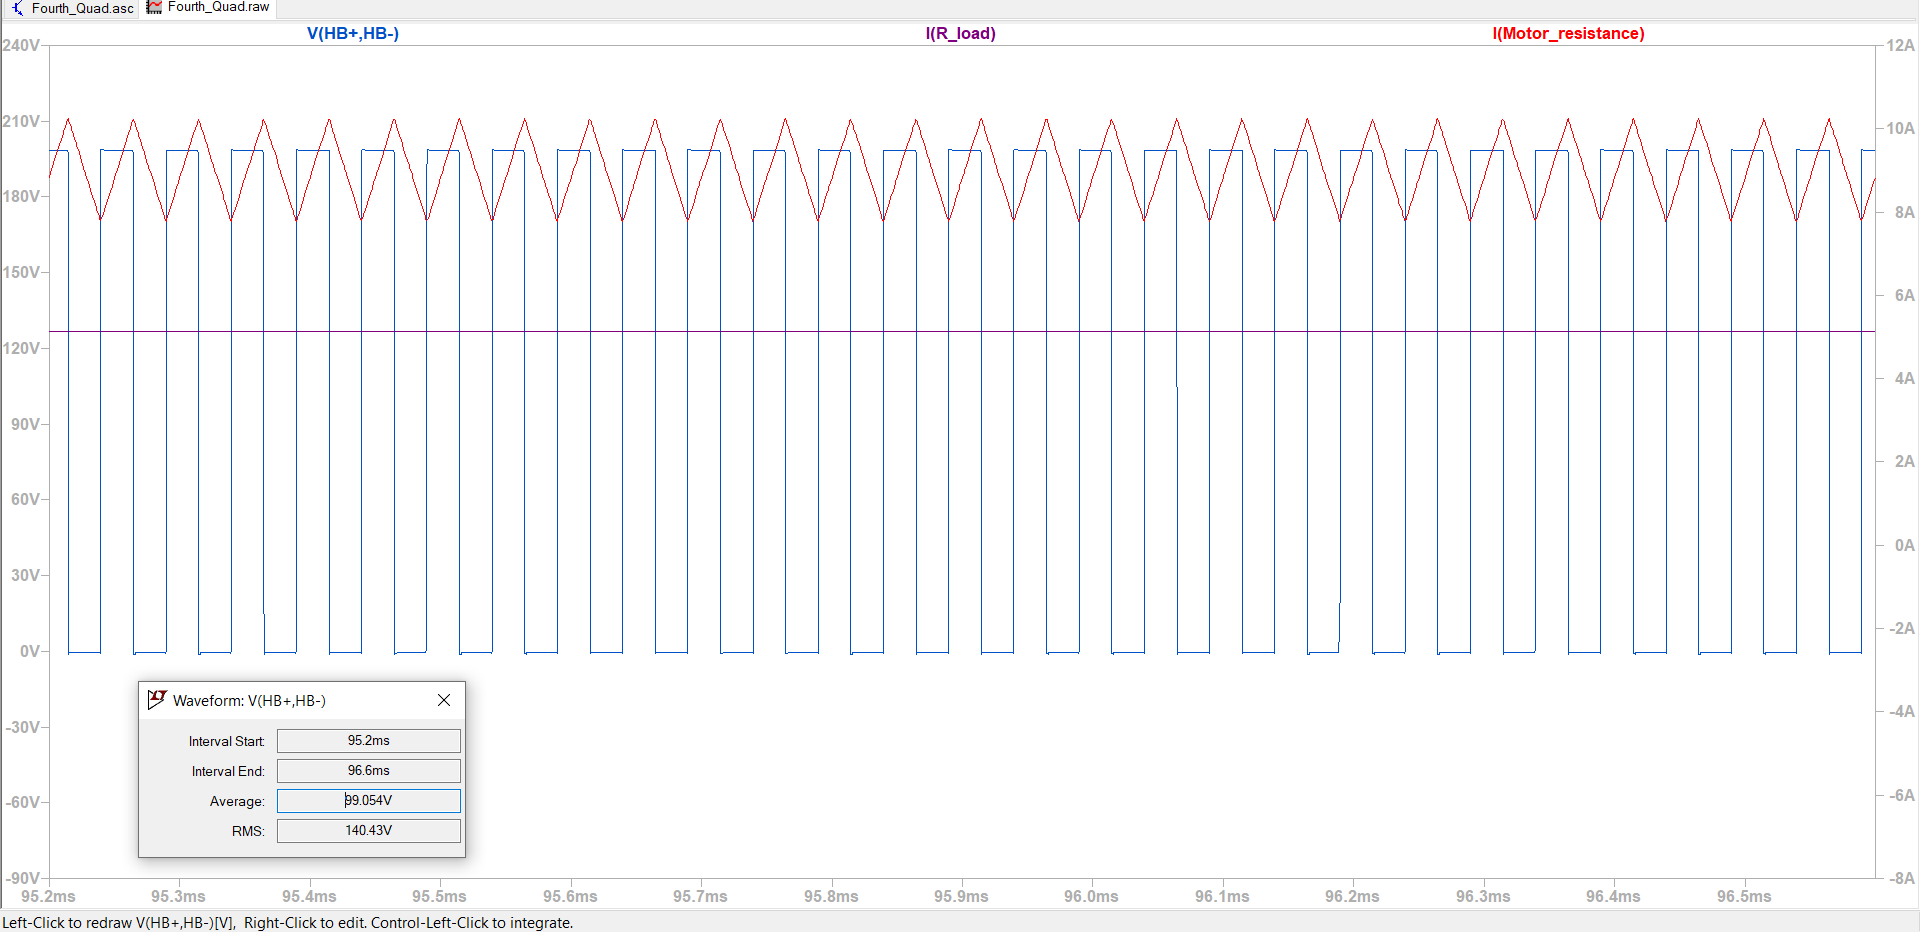
\includegraphics[width=0.8\textwidth]{Figures/Spice_Figures/Motoring_Half_Duty_Sim_1.PNG}
    \caption{Forward motoring simulation for 50\% duty}
    \label{fig:LTspice_forward_50_duty}
\end{figure}

All these simulations are also done with a rectified input, which is coming from a three phase full bridge rectifier. Forward motoring simulation results for the rectified input voltage is given in Figure \ref{fig:LTspice_forward_90_duty_rectified}. Note that there is a significant current ripple in steady state, which is not desired. This will be avoided by the closed loop PID current control by changing the duty according to the input voltage.\\

The average power plots for the output of the driver and one of the switching MOSFETs (M1) are given in Figure \ref{fig:LTspice_forward_90_duty_rectified_power}. The average power consumed by the MOSFET is also calculated and found to be around 10W. This value does not accurately model the real losses, but still gives an idea about the order of magnitude of the MOSFET losses, which is very satisfying for this simulation. In future simulations, more realistic thermal models and simulations will be made.

\begin{figure}[H]
    \centering
    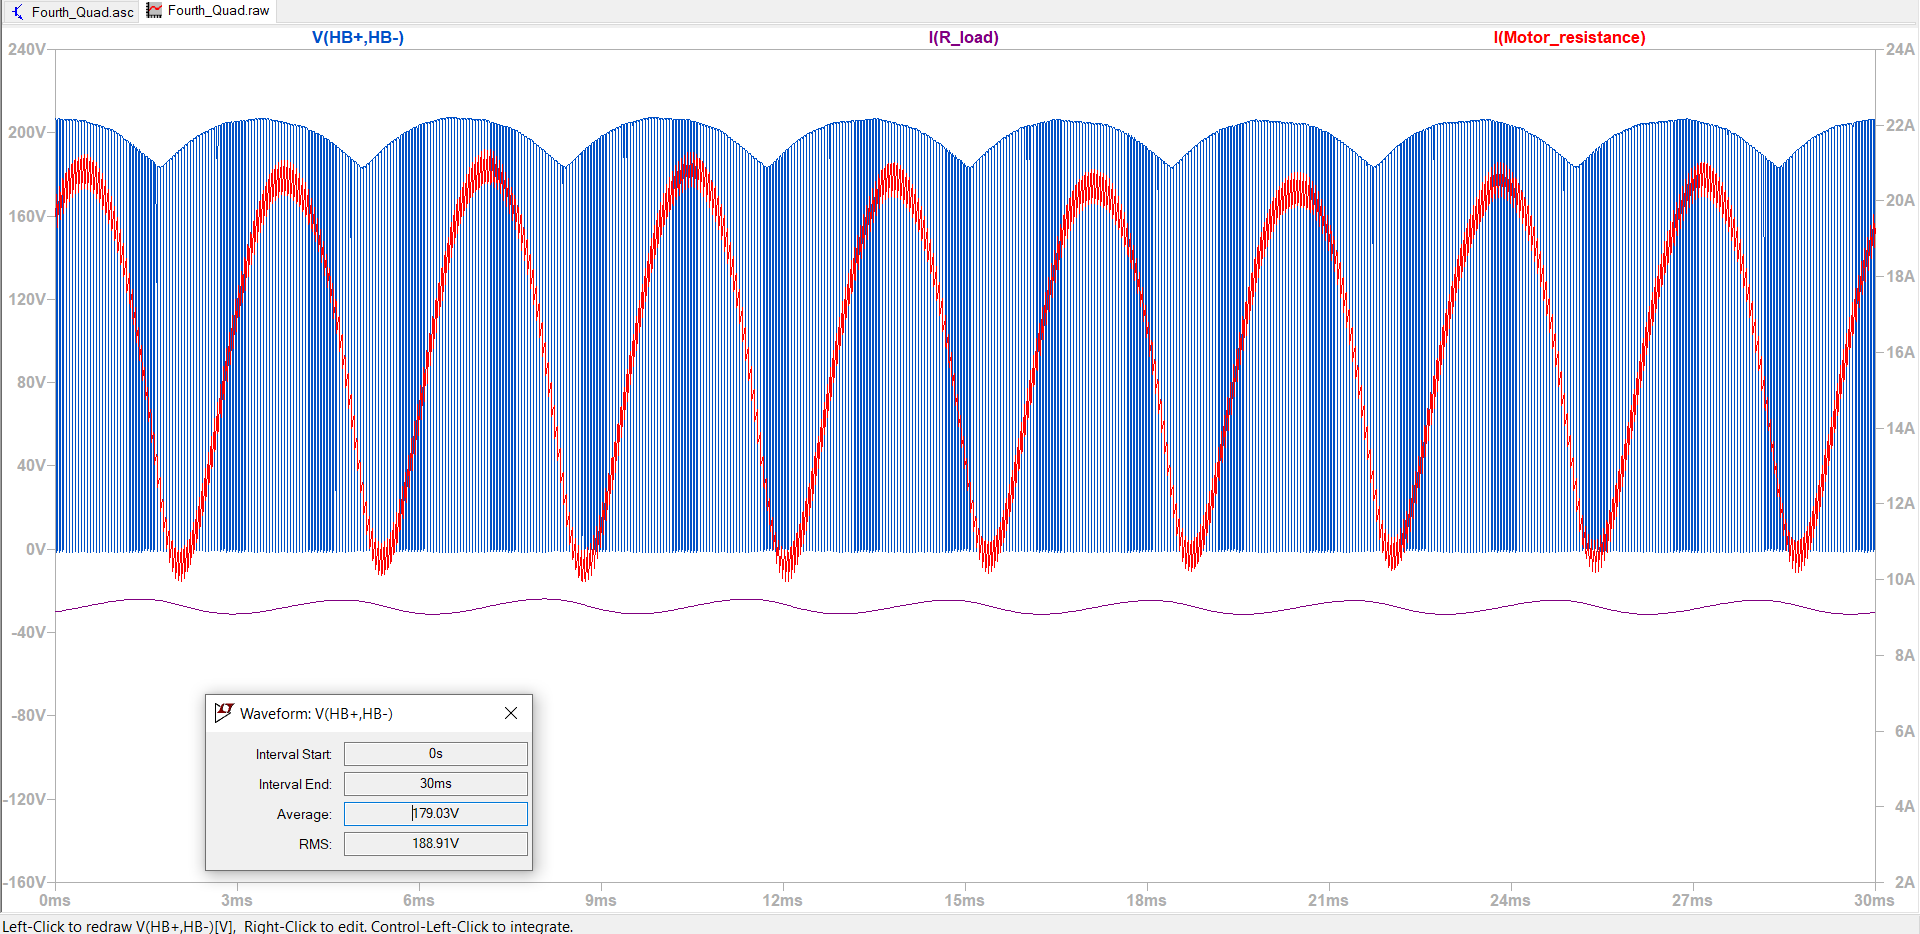
\includegraphics[width=0.8\textwidth]{Figures/Spice_Figures/Motoring_Full_Duty_Rectified_Sim.PNG}
    \caption{Forward motoring simulation for 90\% duty with rectified input}    \label{fig:LTspice_forward_90_duty_rectified}
\end{figure}

\begin{figure}[H]
    \centering
    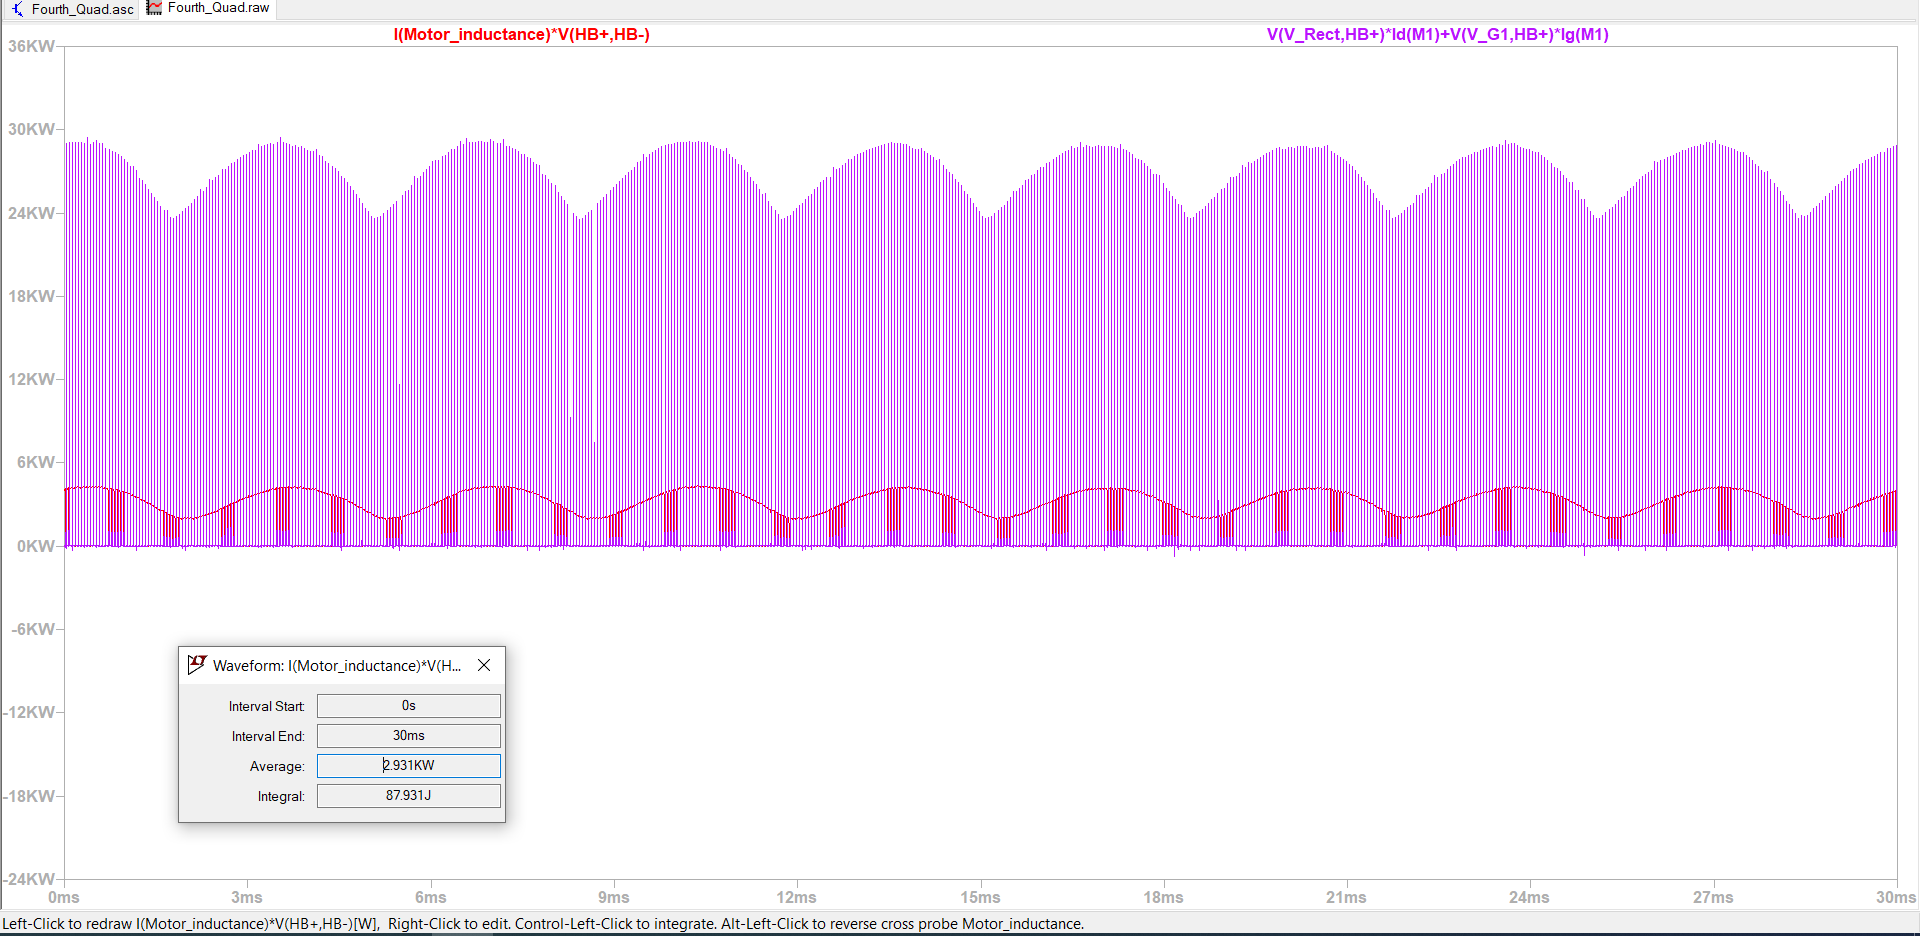
\includegraphics[width=0.8\textwidth]{Figures/Spice_Figures/Motoring_Full_Duty_Rectified_Losses_MOSFET10W_Sim.PNG}
    \caption{Forward motoring simulation for 90\% duty with rectified input, power plots}
    \label{fig:LTspice_forward_90_duty_rectified_power}
\end{figure}

For testing both the forward motoring and regenerative breaking, we made a simulation in which we suddenly change the duty from 90\% to 50\%. This will try to slow down the motor and the motor will release its dissipate its kinetic energy by supplying power to the driver. At this moment, since we did not switch on the chopper resistor in the simulation, the capacitor on the input side is charged to a large value. The transient response is seen in Figure \ref{fig:LTspice_regenerative_breaking}. Note that when our current sensor senses the reverse current, the micro-controller will switch the chopper resistor on and the energy will be dissipated on the resistor.

\begin{figure}[H]
    \centering
    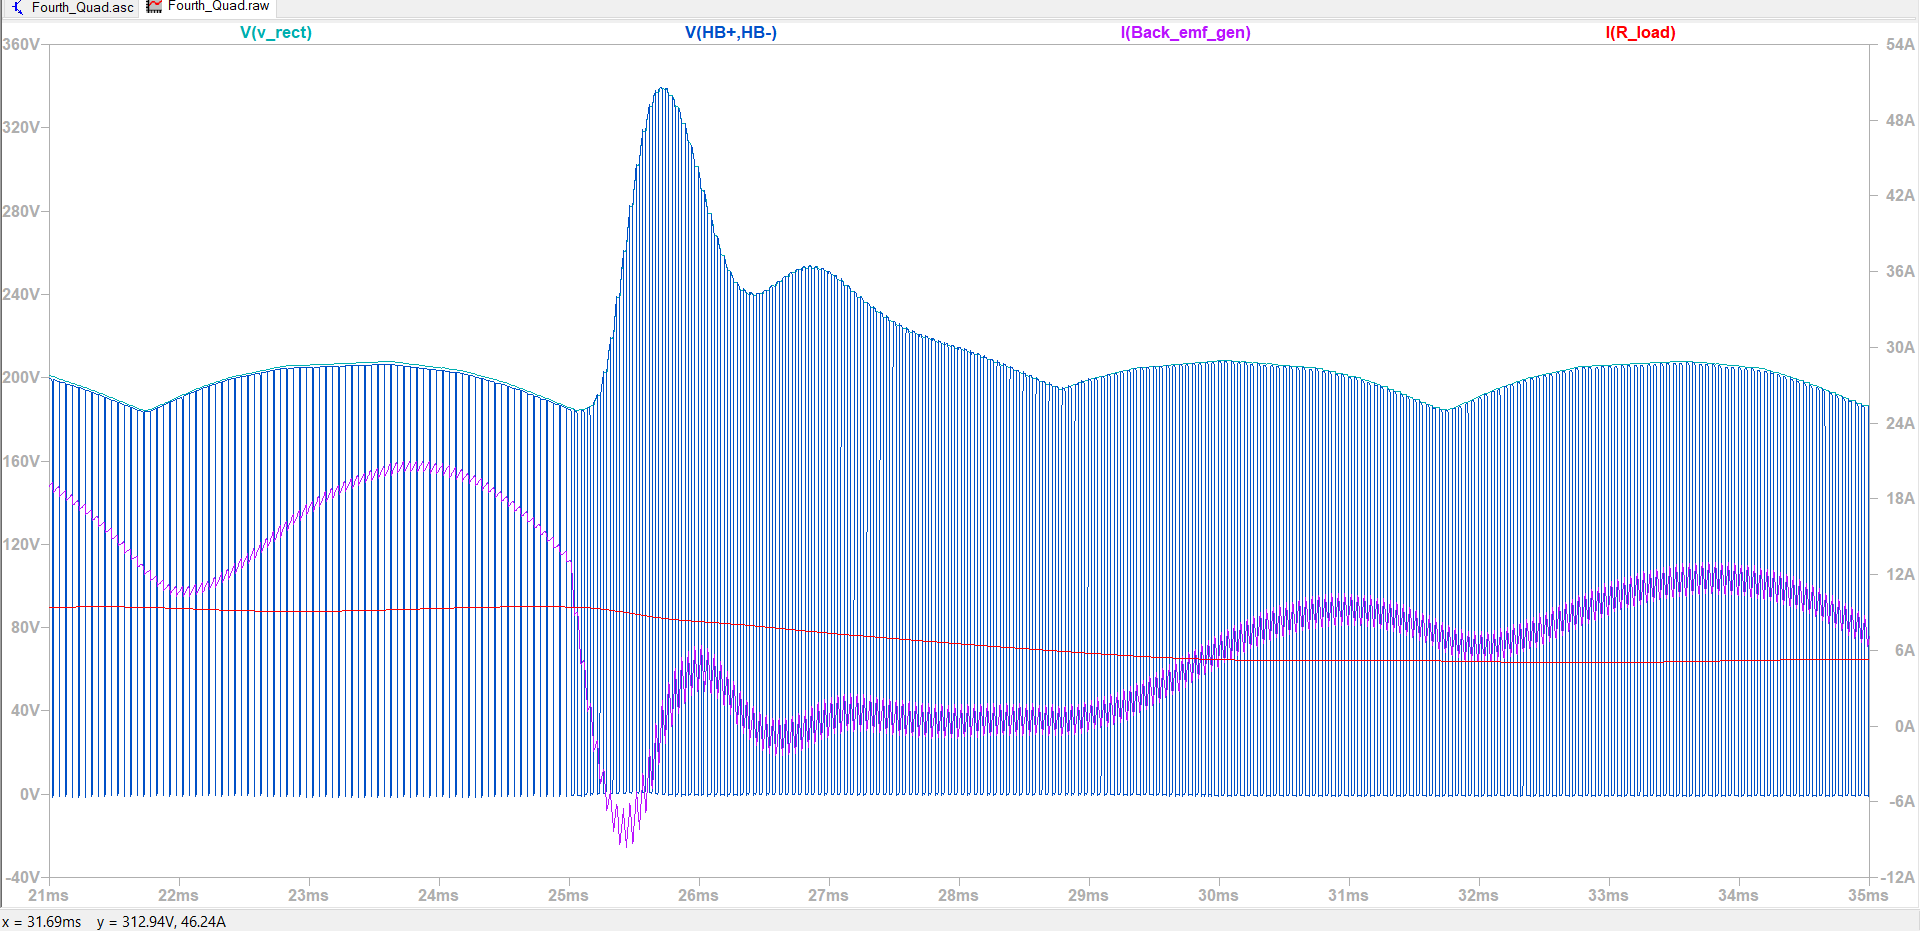
\includegraphics[width=0.8\textwidth]{Figures/Spice_Figures/Motoring_Full_Duty_to_Half_Regenerative_Sim.PNG}
    \caption{Regenerative breaking simulation for sudden slow down (transient)}    
    \label{fig:LTspice_regenerative_breaking}
\end{figure}

The same simulations are run for the reverse motoring operation (M1 off, M2 on, M3 and M4 switched for a synchronous buck with inverted output voltage). The results were similar to the forward motoring case, except for the directions of the currents and voltages on the armature side, which was expected. \\

Finally, the continuous operation in the generation mode is tested by supplying a higher voltage to the other motor. In this operation, none of the MOSFETs are switched on except the chopper switch. The current flow is permitted by the body diodes of the MOSFETs. In the real case, M1 and M4 can be switched to increase the efficiency, but no need to simulate that case. Chopper MOSFET is switched on after 1ms the other motor starts to rotate. The simulation results are given in Figure \ref{fig:LTspice_generation}. One can see that the armature current is negative after the transient, hence supplied to the driver; and the chopper current is positive. These are the desired transient and steady responses of the generation mode and the results are as expected. \\

\begin{figure}[H]
    \centering
    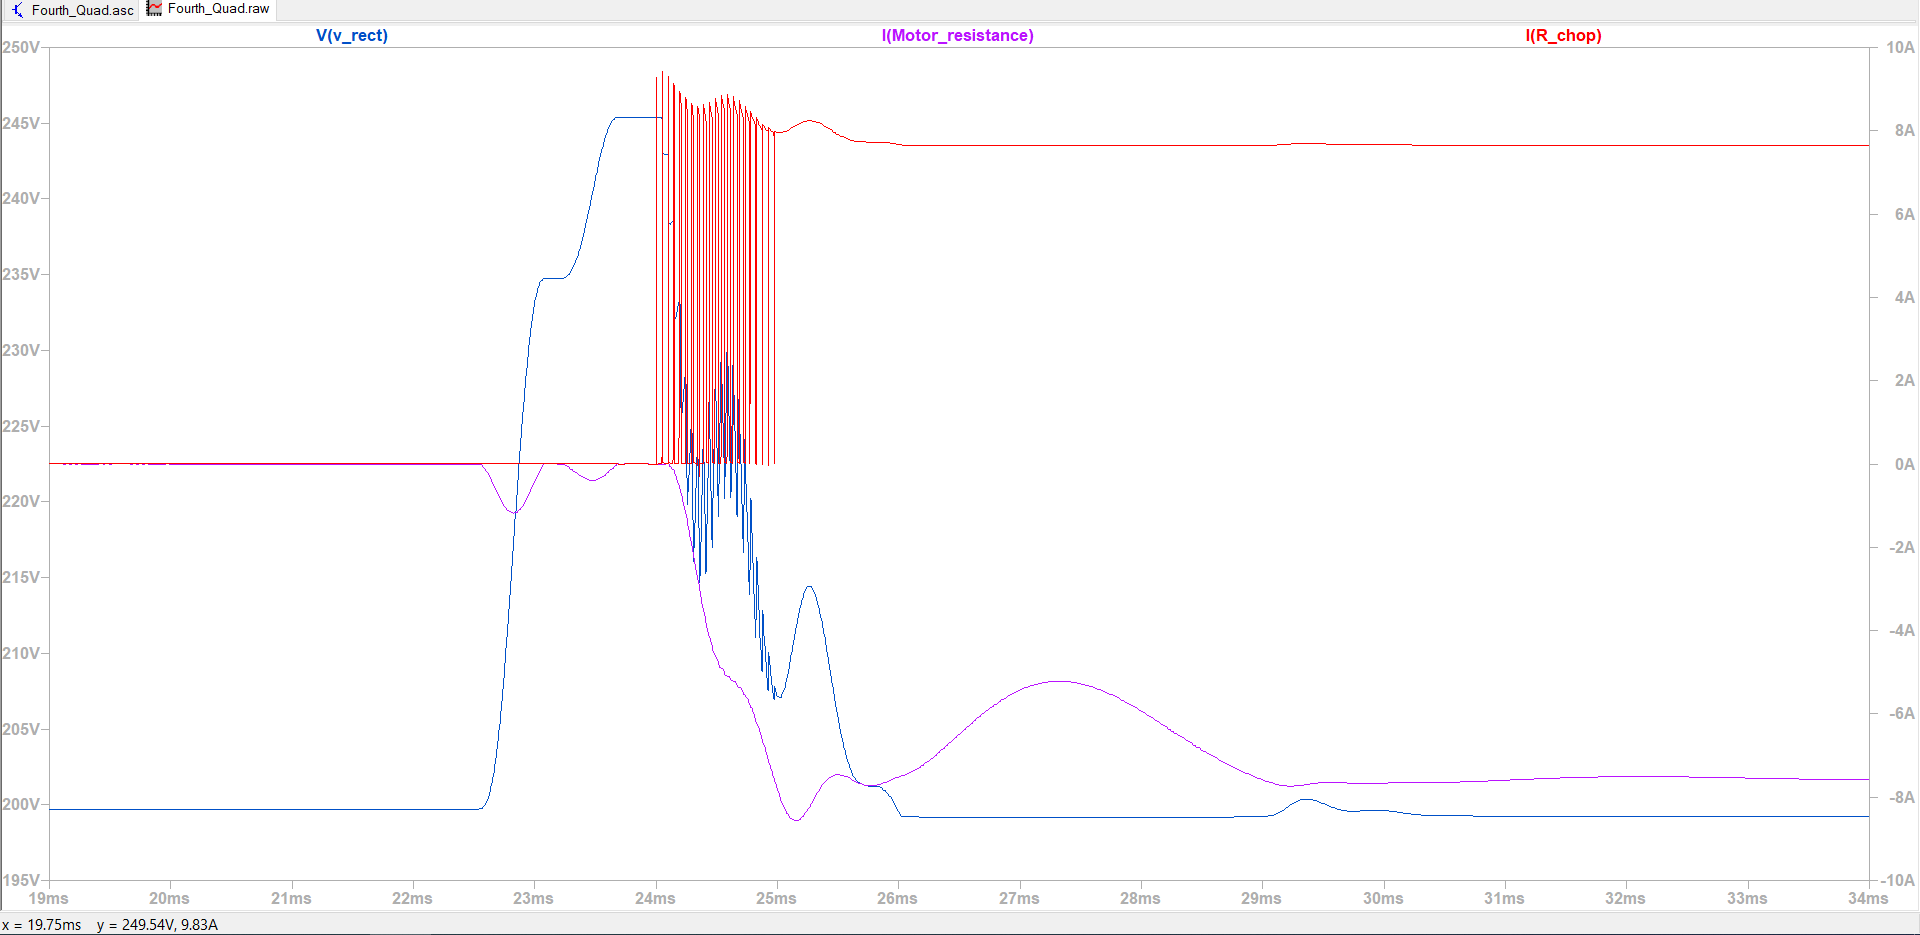
\includegraphics[width=0.8\textwidth]{Figures/Spice_Figures/Generating_Mode_Start.PNG}
    \caption{Continuous generation mode simulation}   
    \label{fig:LTspice_generation}
\end{figure}

In the next steps, we need to consider the inductances and resistances caused by the copper tracks of the PCB layout, which will cause unwanted effects. The realistic models of the components we choose will also be included in the simulations to get better results. Finally, thermal simulations will be conducted according to the directives given by the component manufacturers to further investigate the thermal properties of the system. We continuously update and iterate our simulations to obtain a better view of the electrical, thermal, and mechanical systems considered in our project. For now, we have seen that using H-Bridge topology, we can operate our DC motor in all 4-quadrants with great success.


\subsection{MATLAB Simulations}
Expected circuitry is simulated using MATLAB/Simulink environment. The first stage is added as a three-phase full-bridge rectifier. After that H-bridge and motor simulations are added to have a complete simulation. Simulation setup can be seen in Figures \ref{fig:matlab_model1} \&
\ref{fig:matlab_model2}.

\begin{figure}[ht]
    \centering
    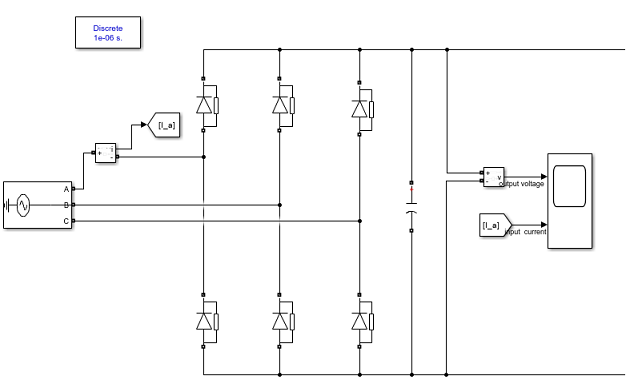
\includegraphics[width=0.8\textwidth]{matlab/MATLAB_model_rect.png}
    \caption{MATLAB Simulation Model Three-Phase FBDR.}
    \label{fig:matlab_model1}
\end{figure}

\begin{figure}[ht]
    \centering
    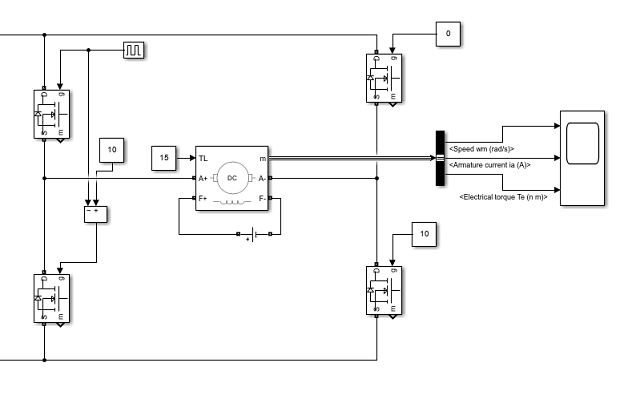
\includegraphics[width=0.8\textwidth]{matlab/MATLAB_model_hbrid.png}
    \caption{MATLAB Simulation Model H-Bridge}
    \label{fig:matlab_model2}
\end{figure}

In this simulation setup, phase-to-phase voltages are given as 150 $V_{rms}$. The output is around 200 $V_{rms}$ with 20 $V_{pp}$ ripple. The H-bridge and DC motor are driven with the output of a three-phase full bridge diode rectifier. Separate simulations are run for motoring, reverse motoring, and regenerative braking modes of operation. In forward motoring, the system works as a synchronous DC-DC buck converter. The output of the forward motoring can be seen in the 50 percent duty cycle in Figure \ref{fig:forward_mot}. The output current is observed to be too much for the system. This is because there is no soft starter simulated. The control part will be implemented later.

\begin{figure}[ht]
    \centering
    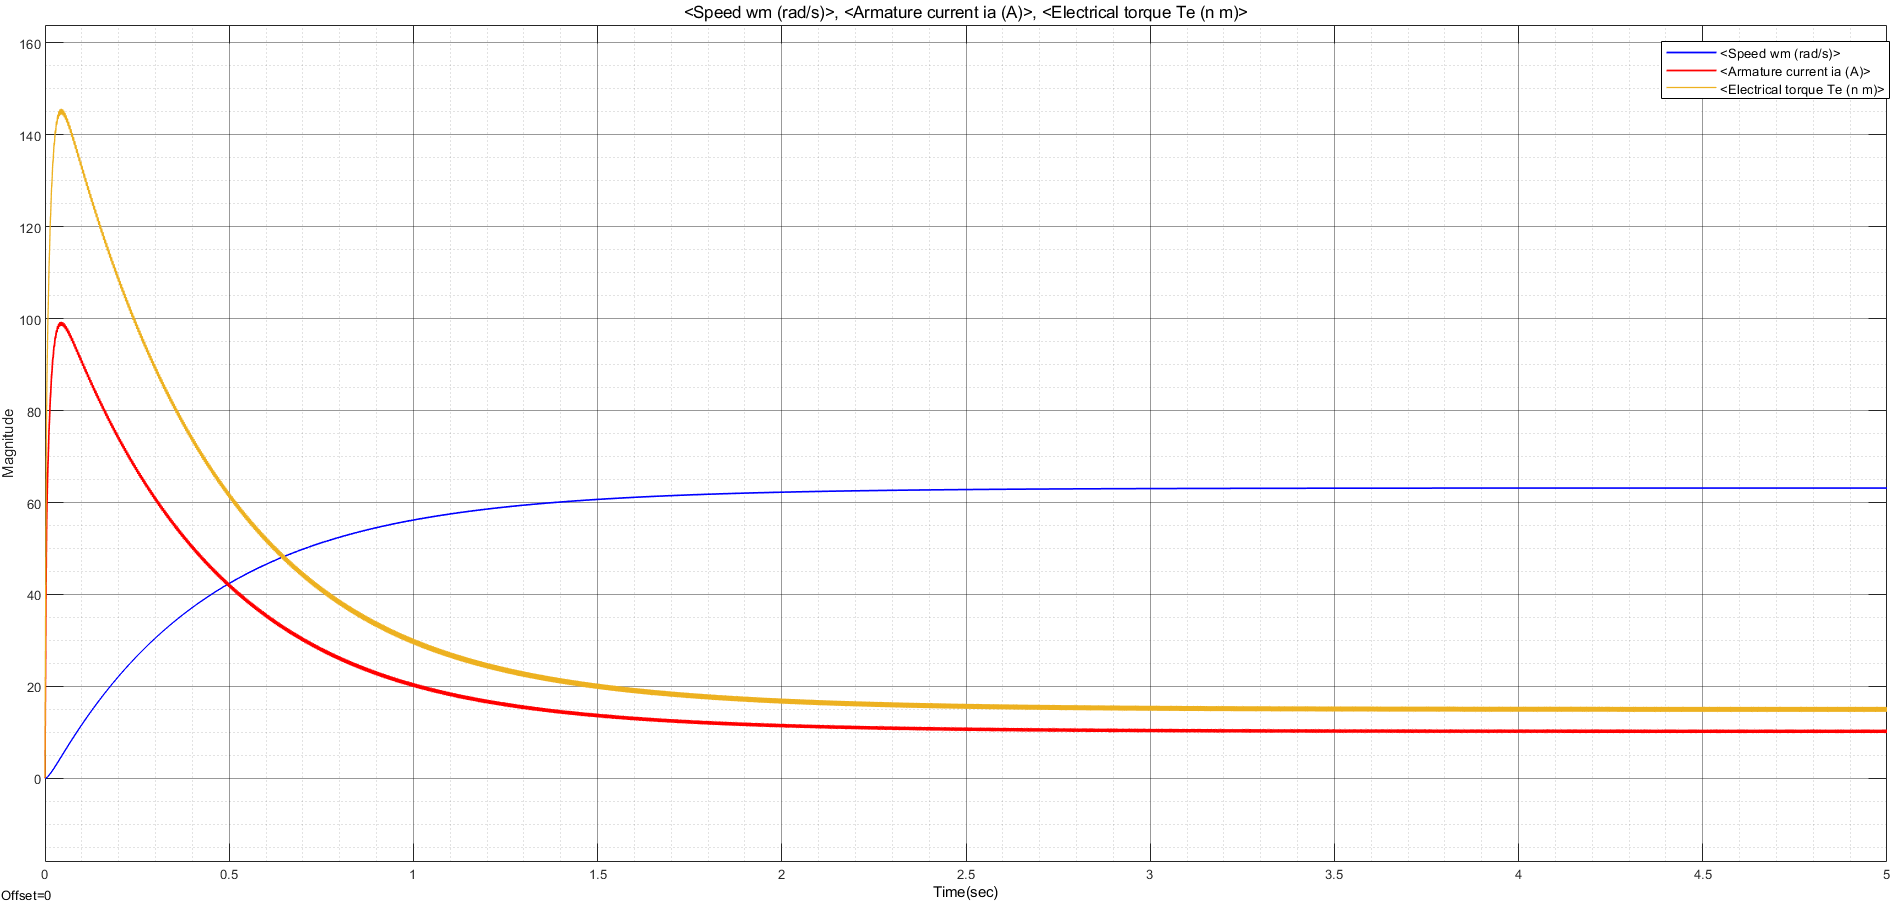
\includegraphics[width=1\textwidth]{matlab/forward motoring D50_900W.png}
    \caption{H-Bridge and DC Motor Simulation at D=0.5 - Forward Motoring}
    \label{fig:forward_mot}
\end{figure}

In Figure \ref{fig:rev_mot}, we see the reverse motoring graph of the motor. It is just the inverted version of forward motoring. The system works with the same logic; however, the controlled MOSFETs are changed due to change of operation. 
\begin{figure}[ht]
    \centering
    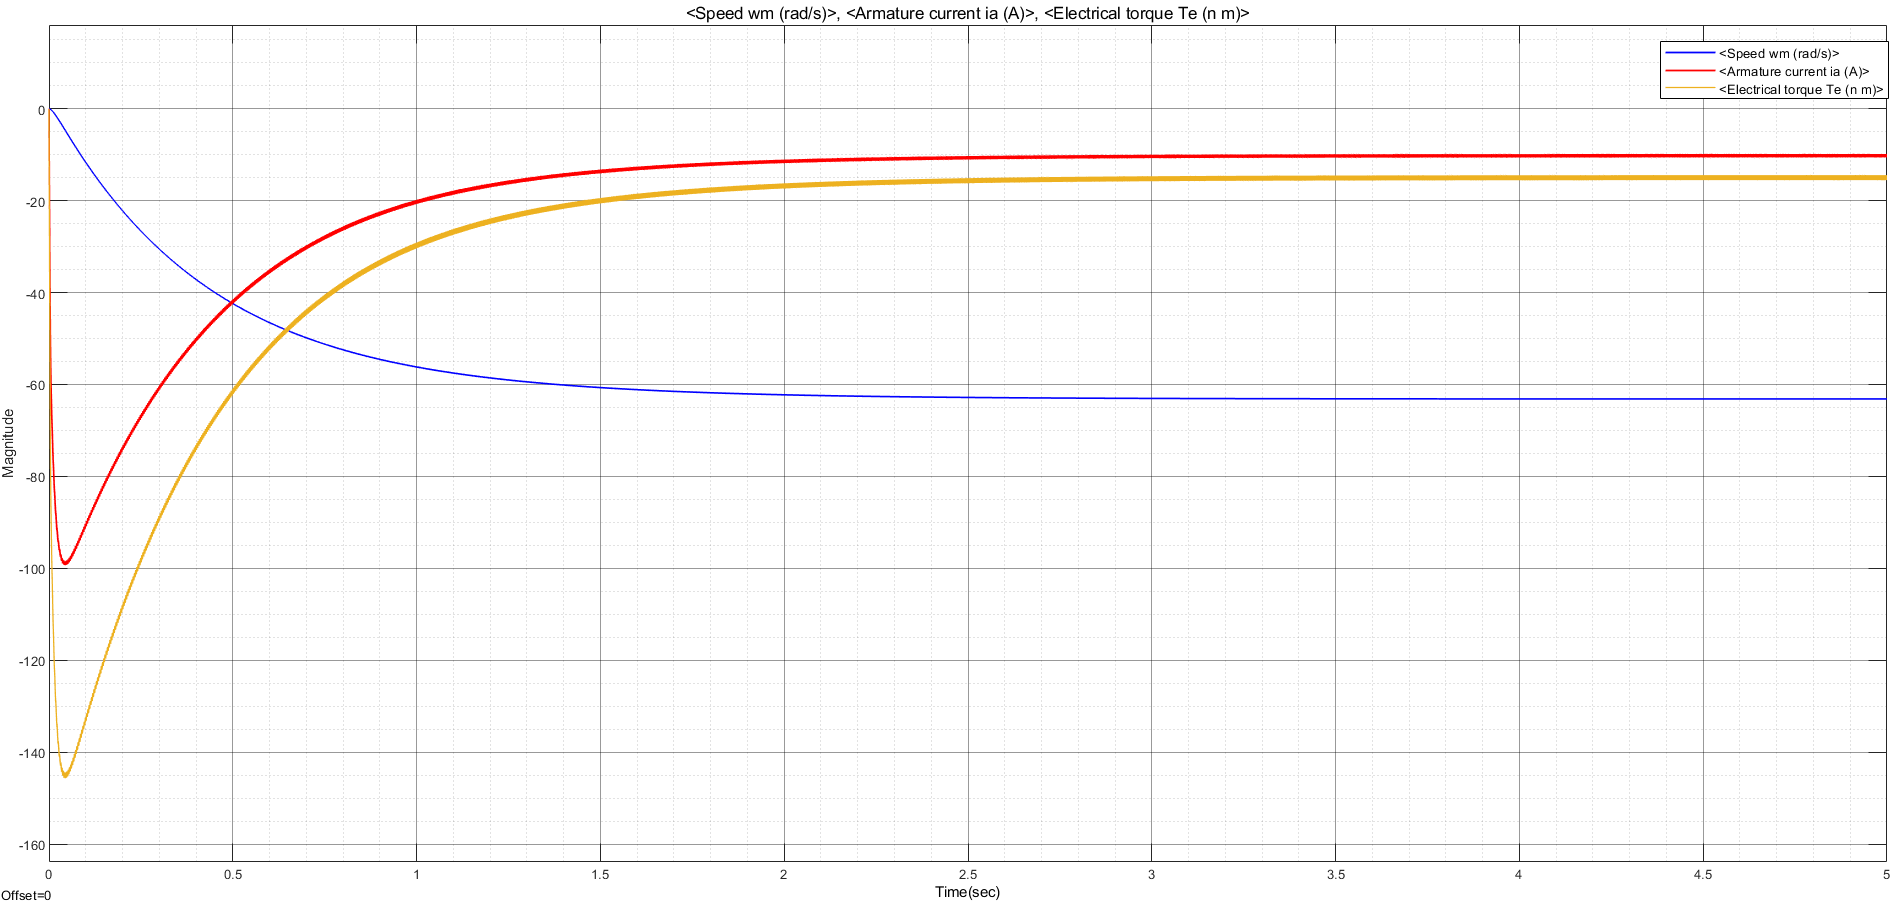
\includegraphics[width=1\textwidth]{matlab/reverse motoring D50_ 900W.png}
    \caption{H-Bridge and DC Motor Simulation at D=0.5 - Reverse Motoring}
    \label{fig:rev_mot}
\end{figure}

The intention of using an H-bridge is to be able to have the four-quadrant drive. More on that topic is explained in Design Decisions[\ref{design}]. The other operation quadrants are braking regions. Braking is simulated in the model by adding a resistor and another MOSFET parallel to the rectifier output as in Figure \ref{fig:braking}.
\newpage
\begin{figure}[ht]
    \centering
    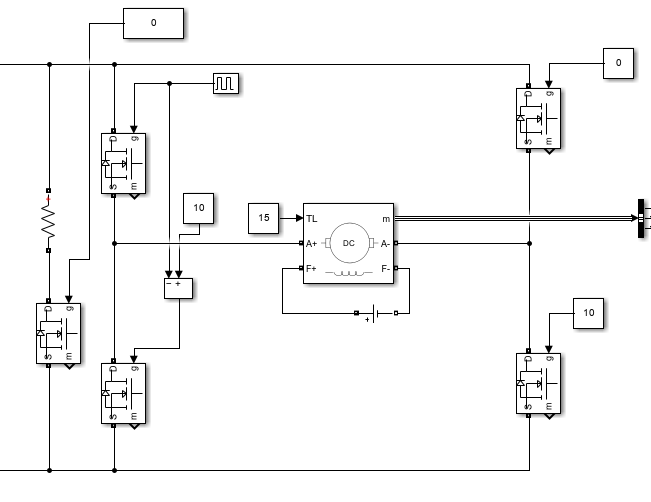
\includegraphics[width=0.8\textwidth]{matlab/braking_added.png}
    \caption{Braking Mode Added Circuitry}
    \label{fig:braking}
\end{figure}

In regenerative braking, the intention is usually to charge a battery system connected to the motor. We will dissipate this external motor energy using a chopper resistor. When it is in braking mode we turn on our MOSFET. More on the operation of the braking mode is explained in Design Decisions[see \ref{design}].

Figure \ref{fig:duty_braking} shows that the current gets below zero, which means our motor injects current into the other direction. This change in the current increases the voltage if not dissipated properly.
\begin{figure}[ht]
    \centering
    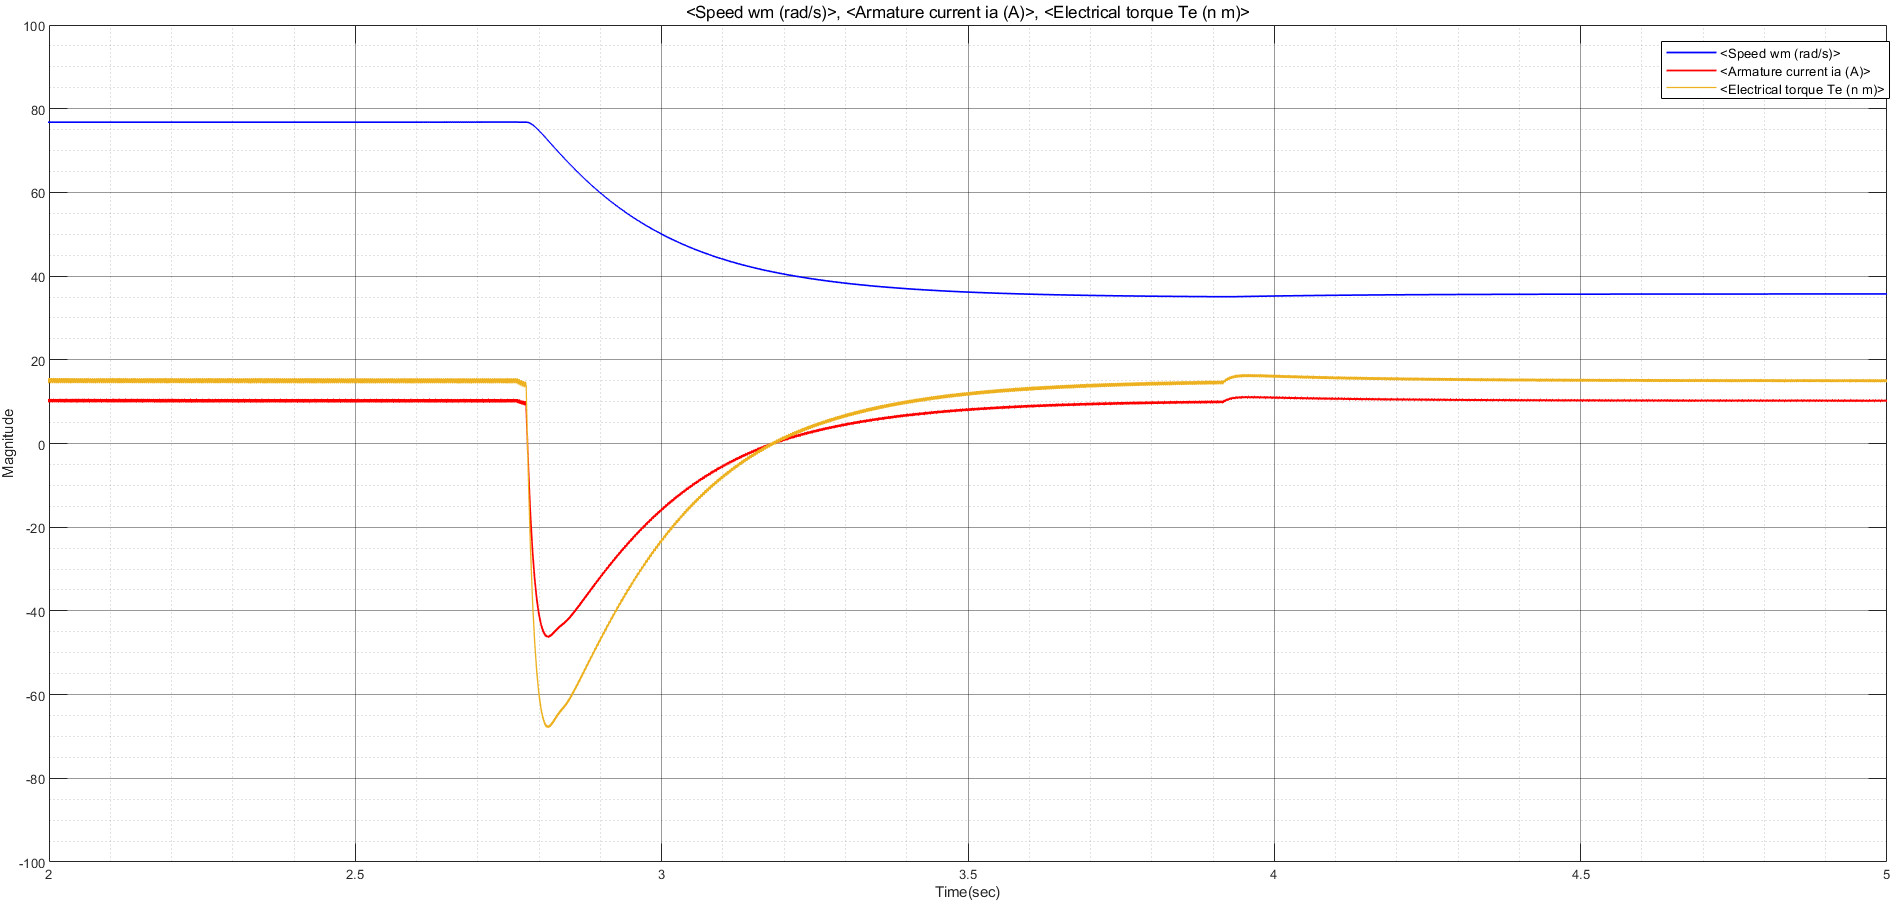
\includegraphics[width=0.9\textwidth]{matlab/braking D60_D30_v2.png}
    \caption{Forward Braking from duty cycle D=0.6 to D=0.3 }
    \label{fig:duty_braking}
\end{figure}

\newpage
\section{Component Selection} \label{component}

\subsection{Three-Phase Full Bridge Rectifier}
In the first stage, we need a three-phase rectifier. For the three-phase rectifier, we decided to use a three-phase bridge diode similar to the \cite{three-phase_bridge} in Figure \ref{fig:bridge} to rectify the signal with the addition of an appropriately sized capacitor. Necessary constraints are given in the Table \ref{tab:ratings_diode}. If we struggle on the three-phase rectifier, we can also consider turning back to the single-phase version of the topology.

\begin{table}[ht]
    \centering
        \begin{tabular}{|c|c|c|}
        \hline
         Peak Voltage   & Peak Current    & Voltage Ripple  \\ 
        \hline
         210 Vpeak      & 31A             & 20Vpp           \\
        \hline
        \end{tabular}
    \caption{Ratings obtained from the Simulations}
    \label{tab:ratings_diode}
\end{table}

\begin{figure}[ht]
    \centering
    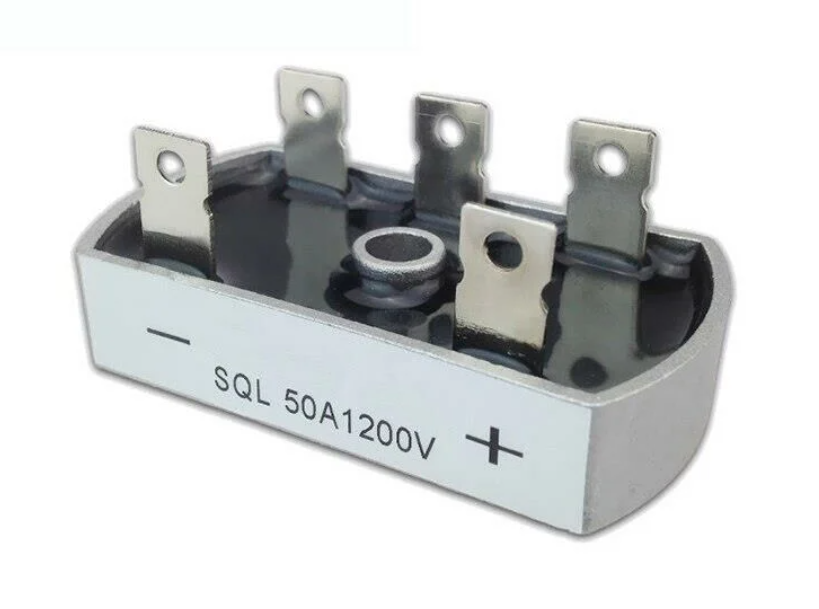
\includegraphics[width=0.4\textwidth]{matlab/bridge_diode.png}
    \caption{Three-phase Full Bridge}
    \label{fig:bridge}
\end{figure}

\subsection{MOSFET Selection}
In MOSFET Selection, transients and peak values play an important role during the switching instants. For conduction modes, continuous current is considered.

\begin{table}[ht]
    \centering
        \begin{tabular}{|c|c|c|}
        \hline
         Peak Voltage   & Peak Current    & Continuous Current  \\
         \hline
         210 V          & 30A             & 10A          \\
        \hline
        \end{tabular}
    \caption{Ratings obtained from the Simulations}
    \label{tab:ratings_DC}
\end{table}

As the voltage rating of the MOSFET increases, the $R_{ds,on}$ resistance of the MOSFET increases. We decided to keep our MOSFETs around the boundaries because we use five of them. 

\begin{table}[ht]
    \centering
        \begin{tabular}{|c|c|c|}
        \hline
         Peak Voltage   & Peak Current    & Continuous Current  \\ 
         \hline
         300 V          & 50A          & 30~40A          \\
        \hline
        \end{tabular}
    \caption{Intended Ratings for MOSFETS}
    \label{tab:ratings_MOS}
\end{table}
There was not enough time to do wide market research for the component selection. Therefore only a few models can be detected initially. Table \ref{tab:selected_MOS} shows some of the possible options. If we can find a model that suits better to our design than the ones given in Table \ref{tab:selected_MOS}, in terms of efficiency, cost and availability, we will consider choosing that model for our design. 

\begin{table}[ht]
    \centering
        \begin{tabular}{|c|c|c|c|c|}
        \hline
         Model   & $V_{ds}$ Voltage(V)    & Continuous Current(A) & $R_{ds,on}(m\Omega)$ & Peak Current(A) \\ 
        \hline
        
         FDAF62N28       &280           &36              &51     &144\\
         FDAF75N28      &280           &46             &51      &184\\
         FDB38N30U       &300           &38             &120     &152\\
         AUIRFP4409     &300            &36             &69     &156\\
         IXFP38N30X3   & 300           & 36            & 34     & 60A\\
         FDA38N30       &300           &38             &70       &150\\ 
         IXTQ52N30P   & 300           & 52            & 66     & 150A\\
         IPB60R060P7ATMA1 &600         &48             &60       &151A\\
           
        \hline
        \end{tabular}
    \caption{Some of the Selected MOSFETs}
    \label{tab:selected_MOS}
\end{table}

\newpage
\section{Conclusion} \label{conclude}

In this report, the first analysis of the selected design for the DC-motor drive, is performed. For the achievement of 4 quadrant operation and ease of control, full-bridge diode rectifier and H-bridge is selected as the design topology. The selected design is compared with other possible topologies for the task based on its advantages and theoretical performances. Simulation of the individual modules are done with some of the non-idealities being present in the simulations. According to the simulation results, rated voltage and current values for different modes of operations, are detected for the components to be implemented in real life application. Appropriate and commercially available diodes, MOSFETs and capacitors are selected for the implementation step of the project.

In the next steps of the project, the most suitable and commercially available ones from the selected models (also new models found recently in the further market research), will be bought. After checking the detailed simulation of these models (including non-idealities of the models to the simulation as much as possible), the implementation phase will start and considering the project specifications, design deliverables and test requirements, design will be modified until the end of the implementation phase of the project.

\newpage
\bibliographystyle{IEEEtran}
\bibliography{ref.bib}

%\newpage
%\section{APPENDIX} \label{appendix}

\end{document}
